\documentclass[12pt]{article}

\usepackage[danish]{babel}
\usepackage{latexsym, amsfonts, amssymb, amsthm, amsmath}
\usepackage{siunitx}
\usepackage{graphicx, pgfplots}
\usepackage{sagetex}

%loaded last
\usepackage[hidelinks]{hyperref}

\sisetup{exponent-product = \cdot,
  output-decimal-marker = {,}}

%Giles Castelles incfig
\usepackage{import}
\usepackage{xifthen}
\usepackage{pdfpages}
\usepackage{transparent}

\newcommand{\incfig}[2][1]{%
  \def\svgwidth{#1\columnwidth}
  \import{../figures/}{#2.pdf_tex}
}

\setlength{\parindent}{0in}
\setlength{\oddsidemargin}{0in}
\setlength{\textwidth}{6.5in}
\setlength{\textheight}{8.8in}
\setlength{\topmargin}{0in}
\setlength{\headheight}{18pt}

\pgfplotsset{compat=newest}

\pgfplotsset{every axis/.append style={
  axis x line=middle,    % put the x axis in the middle
  axis y line=middle,    % put the y axis in the middle
  axis line style={<->,color=black}, % arrows on the axis
}}

\title{Opgaver til forlæsning 15}
\author{Noah Rahbek Bigum Hansen}
\date{24. Oktober 2024}

\begin{document}

\maketitle

\section*{Opg. 10.7}

\begin{figure} [ht]
  \centering
  \caption{}
  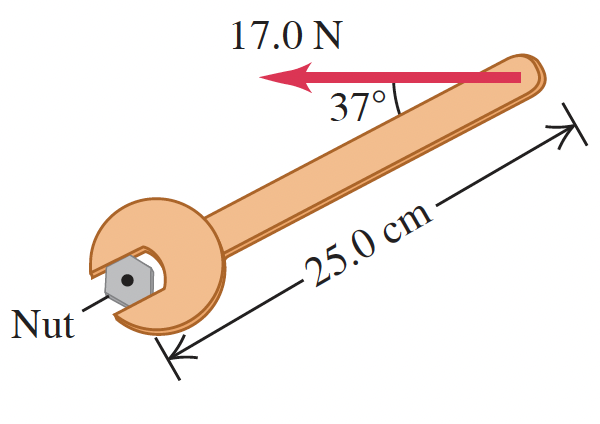
\includegraphics[width=0.35\linewidth]{../figures/E10_7.png}
  \label{fig:E10_7}
\end{figure}

A machinist is using a wrench to loosen a nut. The wrench is \qty{25,0}{cm} long, and he exerts a \qty{17,0}{N} force at the end of the handle at \ang{37} with the handle (\textbf{\autoref{fig:E10_7}}). 

\subsection*{(a)}
What torque does the machinist exert about the center of the nut?
\bigbreak
Kraftmomentet udført på bolten må svare til produktet af kraftens størrelse $|\Vec{F}| =\qty{17,0}{N}$ og den vinkelrette arm fra denne kraft til bolten $|\Vec{r}| = \qty{25,0}{cm}\cdot \sin\left( \ang{37} \right)$. Altså har vi at
\[
  \tau = \qty{17,0}{N}\cdot \qty{25,0}{cm}\cdot  \sin(\ang{37}) = \sage{round(17* 0.25* sin(37*pi/180).n(), 2)} \, \unit{N\cdot m}
.\] 


\subsection*{(b)}
What is the maximum torque he could exert with a force of this magnitude, and how should the force be oriented?
\bigbreak
Det maksimale kraftmoment forekommer idet kraften påvirker svensknøglen vinkelret på bolten. Altså fås at
\[
\tau_{max} = \qty{17,0}{N} \cdot \qty{25,0}{cm} = \sage{round(17*0.25.n(), 2)} \, \unit{N\cdot m}
.\] 


\section*{Opg 10.16}
\begin{figure} [ht]
  \centering
  \caption{}
  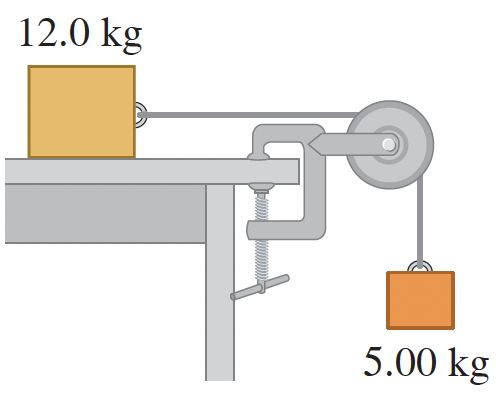
\includegraphics[width=0.35\linewidth]{../figures/E10_16.png}
  \label{fig:E10_16}
\end{figure}

A \qty{12,0}{kg} box resting on a horizontal, frictionless surface is attached to a \qty{5,00}{kg} weight by a thin, light wire that passes over a frictionless pulley (\textbf{\autoref{fig:E10_16}}). The pulley has the shape of a uniform solid disk of mass \qty{2,00}{kg} and diameter \qty{0,500}{m}. After the system is released, find

\subsection*{(a)}
the tension in the wire on both sides of the pulley,
\bigbreak
Vi kan opskrive en række udtryk for systemet. Først opskrives følgende udtryk for spændingen ved klodsen $M = \qty{12,0}{kg}$
\begin{equation}
\sum F_x = T_1 = Ma
\end{equation}
Det samme kan nu gøres for kuglelejet
\begin{equation}
\sum \tau = T_2 R - T_1 R = I\alpha = I \frac{a}{R}
\end{equation}
Og for den sidste klods
\begin{equation}
\sum F_y = mg - T_2 = ma \implies T_2 = m(g-a)
\end{equation}
Kuglelejets inertimoment er givet ved
\begin{equation}
I = \frac{1}{2} \mathcal{M} R^2
\end{equation}
Sætter  vi nu (4) ind i (2) fås
\begin{equation}
T_2 - T_1 = \frac{1}{2}\mathcal{M} a \implies T_2 = (M + \frac{1}{2}\mathcal{M})a
\end{equation}
Sættes (5) ind i (3) fås at
\[
m(g-a) = (M + \frac{1}{2} \mathcal{M})a \implies mg = (m + M + \frac{1}{2}\mathcal{M})a
\]
Altså har vi at
\begin{equation}
a = \frac{m}{m + M + \frac{1}{2}\mathcal{M}}g
\end{equation}
Sættes (6) ind i (1) fås at
\[
T_1 = \frac{Mm}{m+M+\frac{1}{2}\mathcal{M}}g
.\] 
Og sættes (6) ind i (5) fås at
\[
T_2 = T_1 + \frac{1}{2}\mathcal{M}a = (M + \frac{1}{2}\mathcal{M})a = \frac{m(M + \frac{1}{2}\mathcal{M})}{m+M+\frac{1}{2}\mathcal{M}}g
.\] 


\subsection*{(b)}
the acceleration of the box, and
\bigbreak
Accelerationen af kassen er fundet i (6) ovenfor

\subsection*{(c)}
the horizontal and vertical components of the force that the axle exerts on the pulley.
\bigbreak
Den vertikale komponent af kraften må være $\sum F_x = T_1$ og den vertikale komponent er  $\sum T_2 + mg$
  

\section*{Opg. 10.23}
A solid ball is released from rest and slides down a hillside that slopes downward at \ang{65,0} from the horizontal.

\subsection*{(a)}
What minimum value must the coefficient of static friction between the hill and ball surfaces have for no slipping to occur?
\bigbreak
Ved det punkt hvor der netop ikke foretages et glid må det gælde at
\[
f_\mu = F_N \cdot \mu = mg\mu\cdot \cos \alpha
.\]
Fra eksempel 10.7 i bogen har vi i øvrigt at friktionskraften på en bold der ruller ned ad en skråning er
\[
f_\mu = \frac{2}{7}mg \sin \alpha
.\]
Netop der hvor der ikke foretages et glid må disse to størrelser være ens
\[
  mg\mu\cos \alpha = \frac{2}{7}mg \sin \alpha \implies \mu = \frac{2}{7} \tan{\ang{65}} = \sage{round(2/7 * tan(65*pi/180).n(), 2)}
.\] 

\subsection*{(b)}
Would the coefficient of friction calculated in part (a) be sufficient to prevent a hollow ball (such as a soccer ball) from slipping? Justify your answer.
\bigbreak
Inertimomentet af en hul kugle er højere end for en tilsvarende solid kugle og derfor vil summen af moment-infinitesimalerne også være større og derfor ville det kræve en større friktionskraft for at undgå at fodbolden glider.


\subsection*{(c)}
In part (a), why did we use the coefficient of static friction and not the coefficient of kinetic friction?
\bigbreak
Fordi bolden gerne netop skal ligge stille og bolden ligger stadig stille selvom at friktionskraften er større end den dynamiske friktionskraft såfremt bolden var stillestående fra starten af. 


\section*{Opg. 10.30}
\textbf{A Ball Rolling Uphill}. A bowling ball rolls without slipping up a ramp that slopes upward at an angle $\beta$ to the horizontal (see Example 10.7 in Section 10.3). Treat the ball as a uniform solid sphere, ignoring the finger holes. 

\subsection*{(a)}
Draw the free-body diagram for the ball. Explain why the friction force must be directed uphill.
\bigbreak
\begin{figure}[ht]
  \centering
  \incfig[0.5]{E10_30}
  \caption{Fritlegemediagram for bowlingkuglen der ruller opad bakken}
  \label{fig:E10_30}
\end{figure}


\subsection*{(b)}
What is the acceleration of the center of mass of the ball?
\bigbreak
Af fritlegemediagrammet kan ses at den eneste kraft der påvirker bowlingkuglen gennem massemidtpunktet og som ikke er modvirket $F_{t_y}$ og vha. Newtons 2. lov kan accelerationen da findes som
\[
a = \frac{F}{m} \implies a = \frac{mg \sin (\beta)}{m} = g \sin(\beta)
.\] 


\subsection*{(c)}
What minimum coefficient of static friction is needed to prevent slipping?
\bigbreak
Samme argument som i 10.23 (a) kan bruges til at finde $\mu = \frac{2}{7} \tan(\ang{65}) = \num{0,61}$


\section*{Opg. 10.59}
\begin{figure} [ht]
  \centering
  \caption{}
  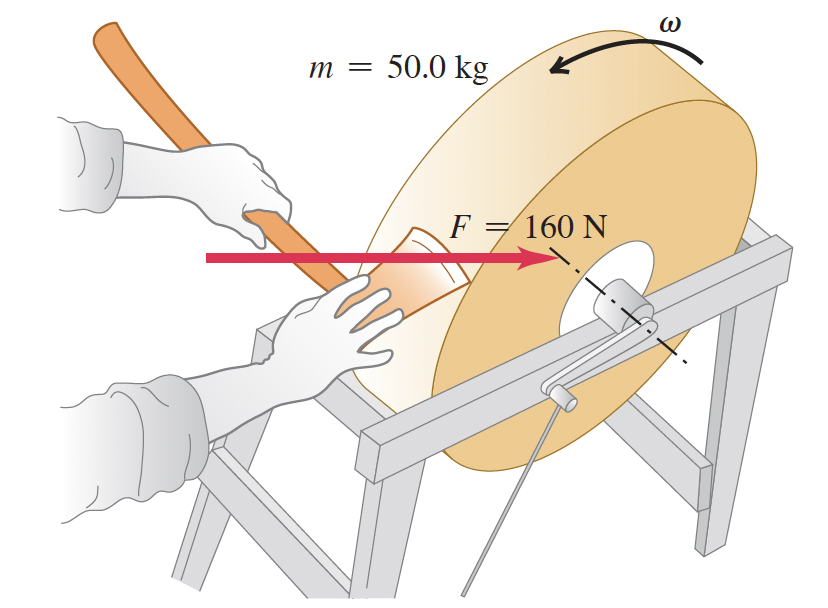
\includegraphics[width=0.35\linewidth]{../figures/P10_58.png}
  \label{fig:P10_58}
\end{figure}

A grindstone in the shape of a solid disk with diameter \qty{0,520}{m} and a mass of \qty{50,0}{kg} is rotating at \qty{850}{rev/min}. You press an ax against the rim with a normal force of \qty{160}{N} (\textbf{\autoref{fig:P10_58}}), and the grindstone comes to rest in \qty{7,50}{s}. Find the coefficient of friction between the ax and the grindstone. You can ignore friction in the bearings.
\bigbreak
Det kraftmoment som er påkrævet for at decelerere stenen må være givet ved
\[
\tau = I\alpha
.\] 
Og den gennemsnitlige vinkelacceleration er 
\[
\alpha = \frac{-\omega_0}{t}
.\] 
Derudover har vi også at
\[
\tau = -F_{\mu}\cdot R = - \mu F_N\cdot R  = -I \frac{\omega_0}{t}
.\] 
Dermed fås at
\begin{align*}
  \mu &= I \frac{\omega_0}{t} \frac{1}{F_N\cdot R} \\
  &= \frac{1}{2}MR^2 \frac{\omega_0}{t} \frac{1}{F_N\cdot R} \\
  &= \frac{1}{2}MR \frac{\omega_0}{t\cdot F_N} \\
  &= \frac{1}{2}\cdot \qty{50,0}{kg}\cdot \qty{0,260}{m} \cdot  \frac{\qty{850}{\frac{rev}{min}}}{\qty{7,50}{s}\cdot \qty{160}{N}} = \num{0,482} \\
.\end{align*}

\section*{Opg. 10.63}
\begin{figure} [ht]
  \centering
  \caption{}
  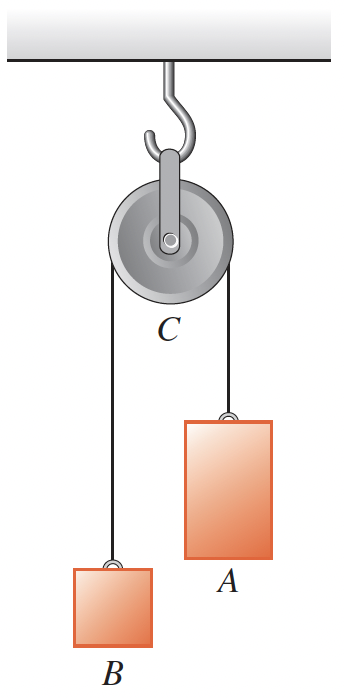
\includegraphics[width=0.15\linewidth]{../figures/P10_63.png}
  \label{fig:P10_63}
\end{figure}

\textbf{The Atwood’s Machine.} (\textbf{\autoref{fig:P10_63}}) illustrates an Atwood’s machine. Find the linear accelerations of blocks $A$ and $B$, the angular acceleration of the wheel $C$, and the tension in each side of the cord if there is no slipping between the cord and the surface of the wheel. Let the masses of blocks $A$ and $B$ be \qty{4,00}{kg} and \qty{2,00}{kg}, respectively, the moment of inertia of the wheel about its axis be \qty{0,220}{kg\cdot m^2}, and the radius of the wheel be \qty{0,120}{m}.

\end{document}
